\documentclass[bibliography=totocnumbered,twocolumn]{scrarticle}
\usepackage{imakeidx}
\usepackage{ragged2e}
\usepackage{setspace} % Um den Zeilenabstand zu ändern.
\usepackage{gensymb}
%\usepackage{authblk}
% \usepackage{minitoc} % for the chpaters
\usepackage{wasysym}
%\usepackage{SI}
\usepackage{array} % Verwendung von Matrizen
\usepackage{booktabs} % Schöne Tabellen beziehungsweise sie sehen damit professioneller aus.
\usepackage{tabulary} % Ähnlich wie tabularx, ermöglicht aber das ändern der Ausrichtung der Spalten.
\usepackage{tabularx} % Tabellen mit automatischen Zeilenumbruch.
\usepackage{enumitem}
\usepackage{physics}
\usepackage[T1]{fontenc}% fontec und inputenc ermöglichen
\usepackage{graphicx}%Für Grafiken
\usepackage{rotating} % lässt Grafiken rotieren
\usepackage{mathtools}% mathematische Werkzeuge
\usepackage{amsmath}% Mathetools
\usepackage{amsfonts}% Mathetools
\usepackage{amssymb}% Symbole wie Natürliche Zahlen
\usepackage{geometry}
%\usepackage{bibtex} 
\usepackage{tablefootnote}% Fußnoten in Tabellen
\usepackage{float}% für eingebundene Bilder
\usepackage{fancyhdr} % Seiten schöner gestalten, insbesondere Kopf- und Fußzeile
\usepackage{ulem} 
\usepackage{dcolumn}% Align table columns on decimal point
\usepackage{bm}% bold math
\usepackage[english]{babel} % Worttrennung nach der neuen Rechtschreibung und deutsche Bezeichnungen. babelfunktion wird wegen Literatur gebraucht.
\usepackage{subfloat} % Was macht diese Packet?
\usepackage{caption} % Unter-/Überschriften für Bilder, Grafiken und Tabellen
\usepackage{subcaption}
\usepackage{txfonts}
\usepackage{titling}% Titel
\usepackage[style=numeric]{biblatex} %biblatex mit alphabetic laden. alphbetic=Zitationsstil
\usepackage{bookmark}
\usepackage[printonlyused]{acronym}
\usepackage{amsthm}
\usepackage{pdfpages}
\usepackage{tikz}
\usepackage[siunitx,americanvoltages, europeanresistors,americancurrents]{circuitikz}
\usepackage{listings}
\usepackage{abstract}
\usepackage[per-mode = fraction]{siunitx}
\usepackage{hyperref}

\newcommand{\R}{\mathbb{R}} % reelle Zahlen
\newcommand{\N}{\mathbb{N}} % natürliche Zahlen
\newcommand{\C}{\mathbb{C}} % komplexe Zahlen
\newcommand{\Q}{\mathbb{Q}} % rationale Zahlen
\newcommand{\Z}{\mathbb{Z}} % ganze Zahlen
\newcommand{\F}{\mathbf{F}} % Kraft
\newcommand{\E}{\mathbf{E}} % Energie
\newcommand{\V}{\mathbf{v}} % Geschwindigkeit
\newcommand{\B}{\mathbf{B}} % magnetischer Fluss
\newcommand{\J}{\mathbf{j}} % Stromdichte ?
\newcommand{\D}{\mathbf{D}} % elektrische Induktion
\newcommand{\HH}{\mathbf{H}} % magnetische Feldstärke
\newcommand{\M}{\mathbf{M}} % Magnetisierung
\newcommand{\p}{\mathbf{P}}
\newcommand{\rr}{\mathbf{r}}
\newcommand{\vp}{\varphi}
\newcommand{\ve}{\varepsilon}
\newcommand{\vcc}[1]{\left(\begin{matrix}#1\end{matrix}  \right)}
\newcommand{\m}[1]{\left\lbrace #1\right\rbrace}
\newcommand{\los}{\noindent\textbf{Lösung}:}
\newcommand{\rang}[2]{\text{Rang}(#1)=#2}
\newcommand{\vpe}{\frac{1}{4\pi\ve_0}}
\newcommand{\qvpe}{\frac{q}{4\pi\ve_0}}
\newcommand{\geg}{\ac{geg.}}
\newcommand{\ges}{\ac{ges.}}

\newcommand{\kommando}[1]{$\backslash$\textit{#1}}
\newcommand{\com}[1]{$\backslash$\textit{#1}$\left\lbrace\ldots\right\rbrace$}
\newcommand{\Com}[2]{$\backslash$\textit{#1}$\left\lbrace #2\right\rbrace$}
\newcommand{\NeuKommando}[2]{$\backslash \textit{#1} \left\lbrace \backslash \textit{#2}\right\rbrace$}
\newcommand{\latex}{\LaTeX $\;$}
\hypersetup{
	colorlinks=true,
	linkcolor=blue,
	filecolor=magenta,      
	urlcolor=red,
	citecolor=lime!50!black,
}
%\addbibresource{} %Bibliographiedateien laden
\addbibresource{Bib.bib}

\geometry{a4paper, left=25mm, right=25mm, top=30mm, bottom=30mm}

\date{\today}
\lhead{\thedate}
\rhead{Modul}
\lhead{\thetitle}
\pagestyle{fancy}
\lfoot{University}

\usetikzlibrary{patterns}
\usetikzlibrary{3d}

\author{Author 1\\(number)\\Mail-address \and Author 2\\(number)\\Mail-address}
\allowdisplaybreaks

\lstset
{ %Formatting for code in appendix
    basicstyle=\footnotesize,
    numbers=left,
    stepnumber=1,
    showstringspaces=false,
    tabsize=2,
    breaklines=true,
    breakatwhitespace=false,
}

\title{Title}
\begin{document}
    \twocolumn[
        \begin{@twocolumnfalse}
            \maketitle
            \begin{abstract}
                
            \end{abstract}
        \end{@twocolumnfalse}
    ]
    \section{Introduction}
        The introduction can be kept very short. In the case of a publication, it serves to classify the work carried out within the research landscape and to prepare the reader who is not a specialist in the subject for the subject matter. It can be assumed that your supervisor does not need this.
        
        \begin{figure}[H]
            \centering
            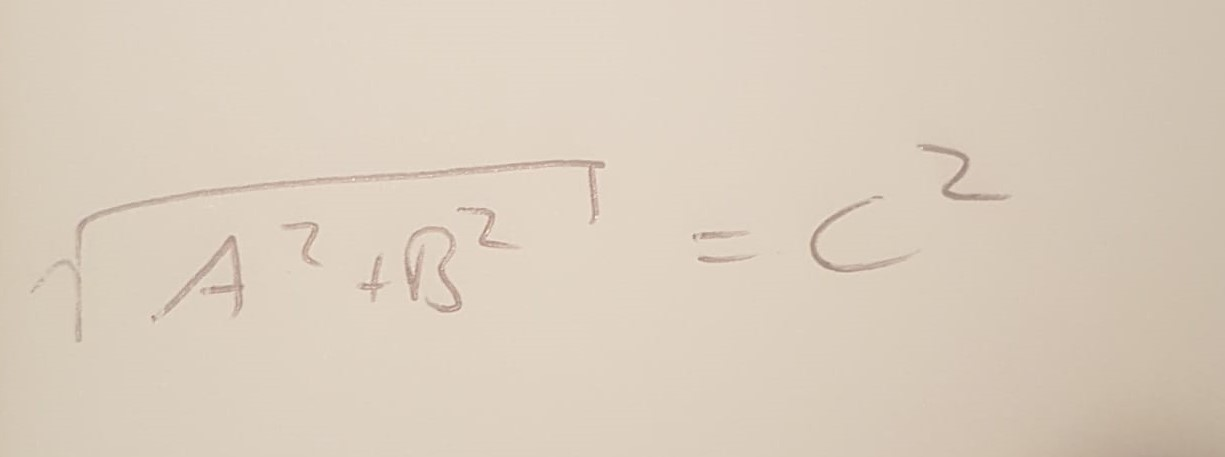
\includegraphics[width=\linewidth]{figures/Template/example.jpeg}
            \caption{Example}
            \label{fig: exp}
        \end{figure}
    \section{Materials and Methods}
        In Materials and Methods, the experimental setups are described, the devices or experimental systems used with type designation and also special procedures for data evaluation/software, if necessary. Again: as short as possible, but the qualified reader should be able to understand your description. Sketches are often useful.
    \newpage
    \section{Analysis and Discussion}
        In evaluation and discussion (often separately in more complex publications), the results are presented and analyzed, discussed in comparison with those in other works and of course the accuracy of the results is assessed. A result without an error statement is not a result and the accuracy of the results should always be visible in a graphic (if necessary error crosses etc.). This section includes the knowledge gained and the consequences thereof.
    \section{Conclusion}
        The conclusions are summarized at the end...again brief, but the well-trained reader should get a rough picture of your work and its results with the abstract and conclusions.
\end{document}